\chapter{Computational Speed Up of RL-MPC}
%\label{chapter:title}

\emph{description of chapter}

\section{Case Study 1 - Reducing Neurons}
\emph{the results and discussion of the effect of reducing the neurons in the value funciton and the effect on computational time and performance}


\begin{figure}[H]
	\centering
	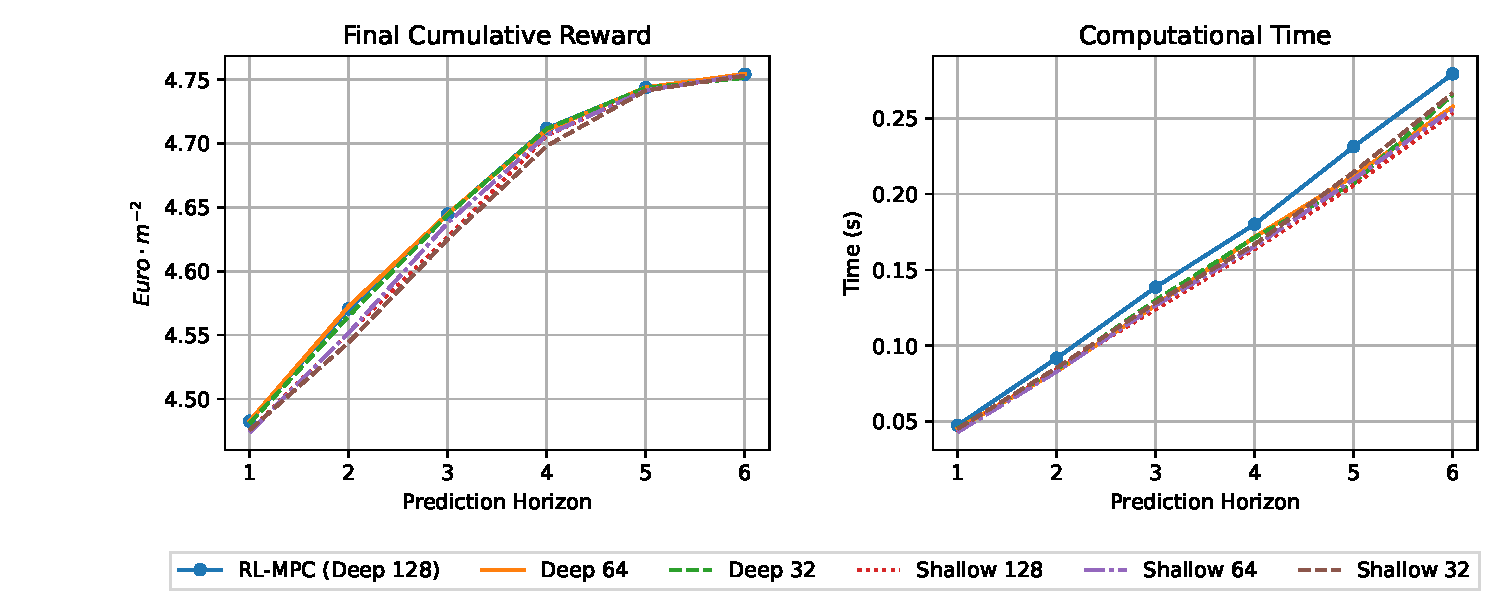
\includegraphics[width=\textwidth]{figures/speed_up_neurons.eps}
	\caption{Fast RL-MPC with Reduced Neurons}
	\label{fig:neurons-speedup}
\end{figure}

\begin{figure}[H]
	\centering
	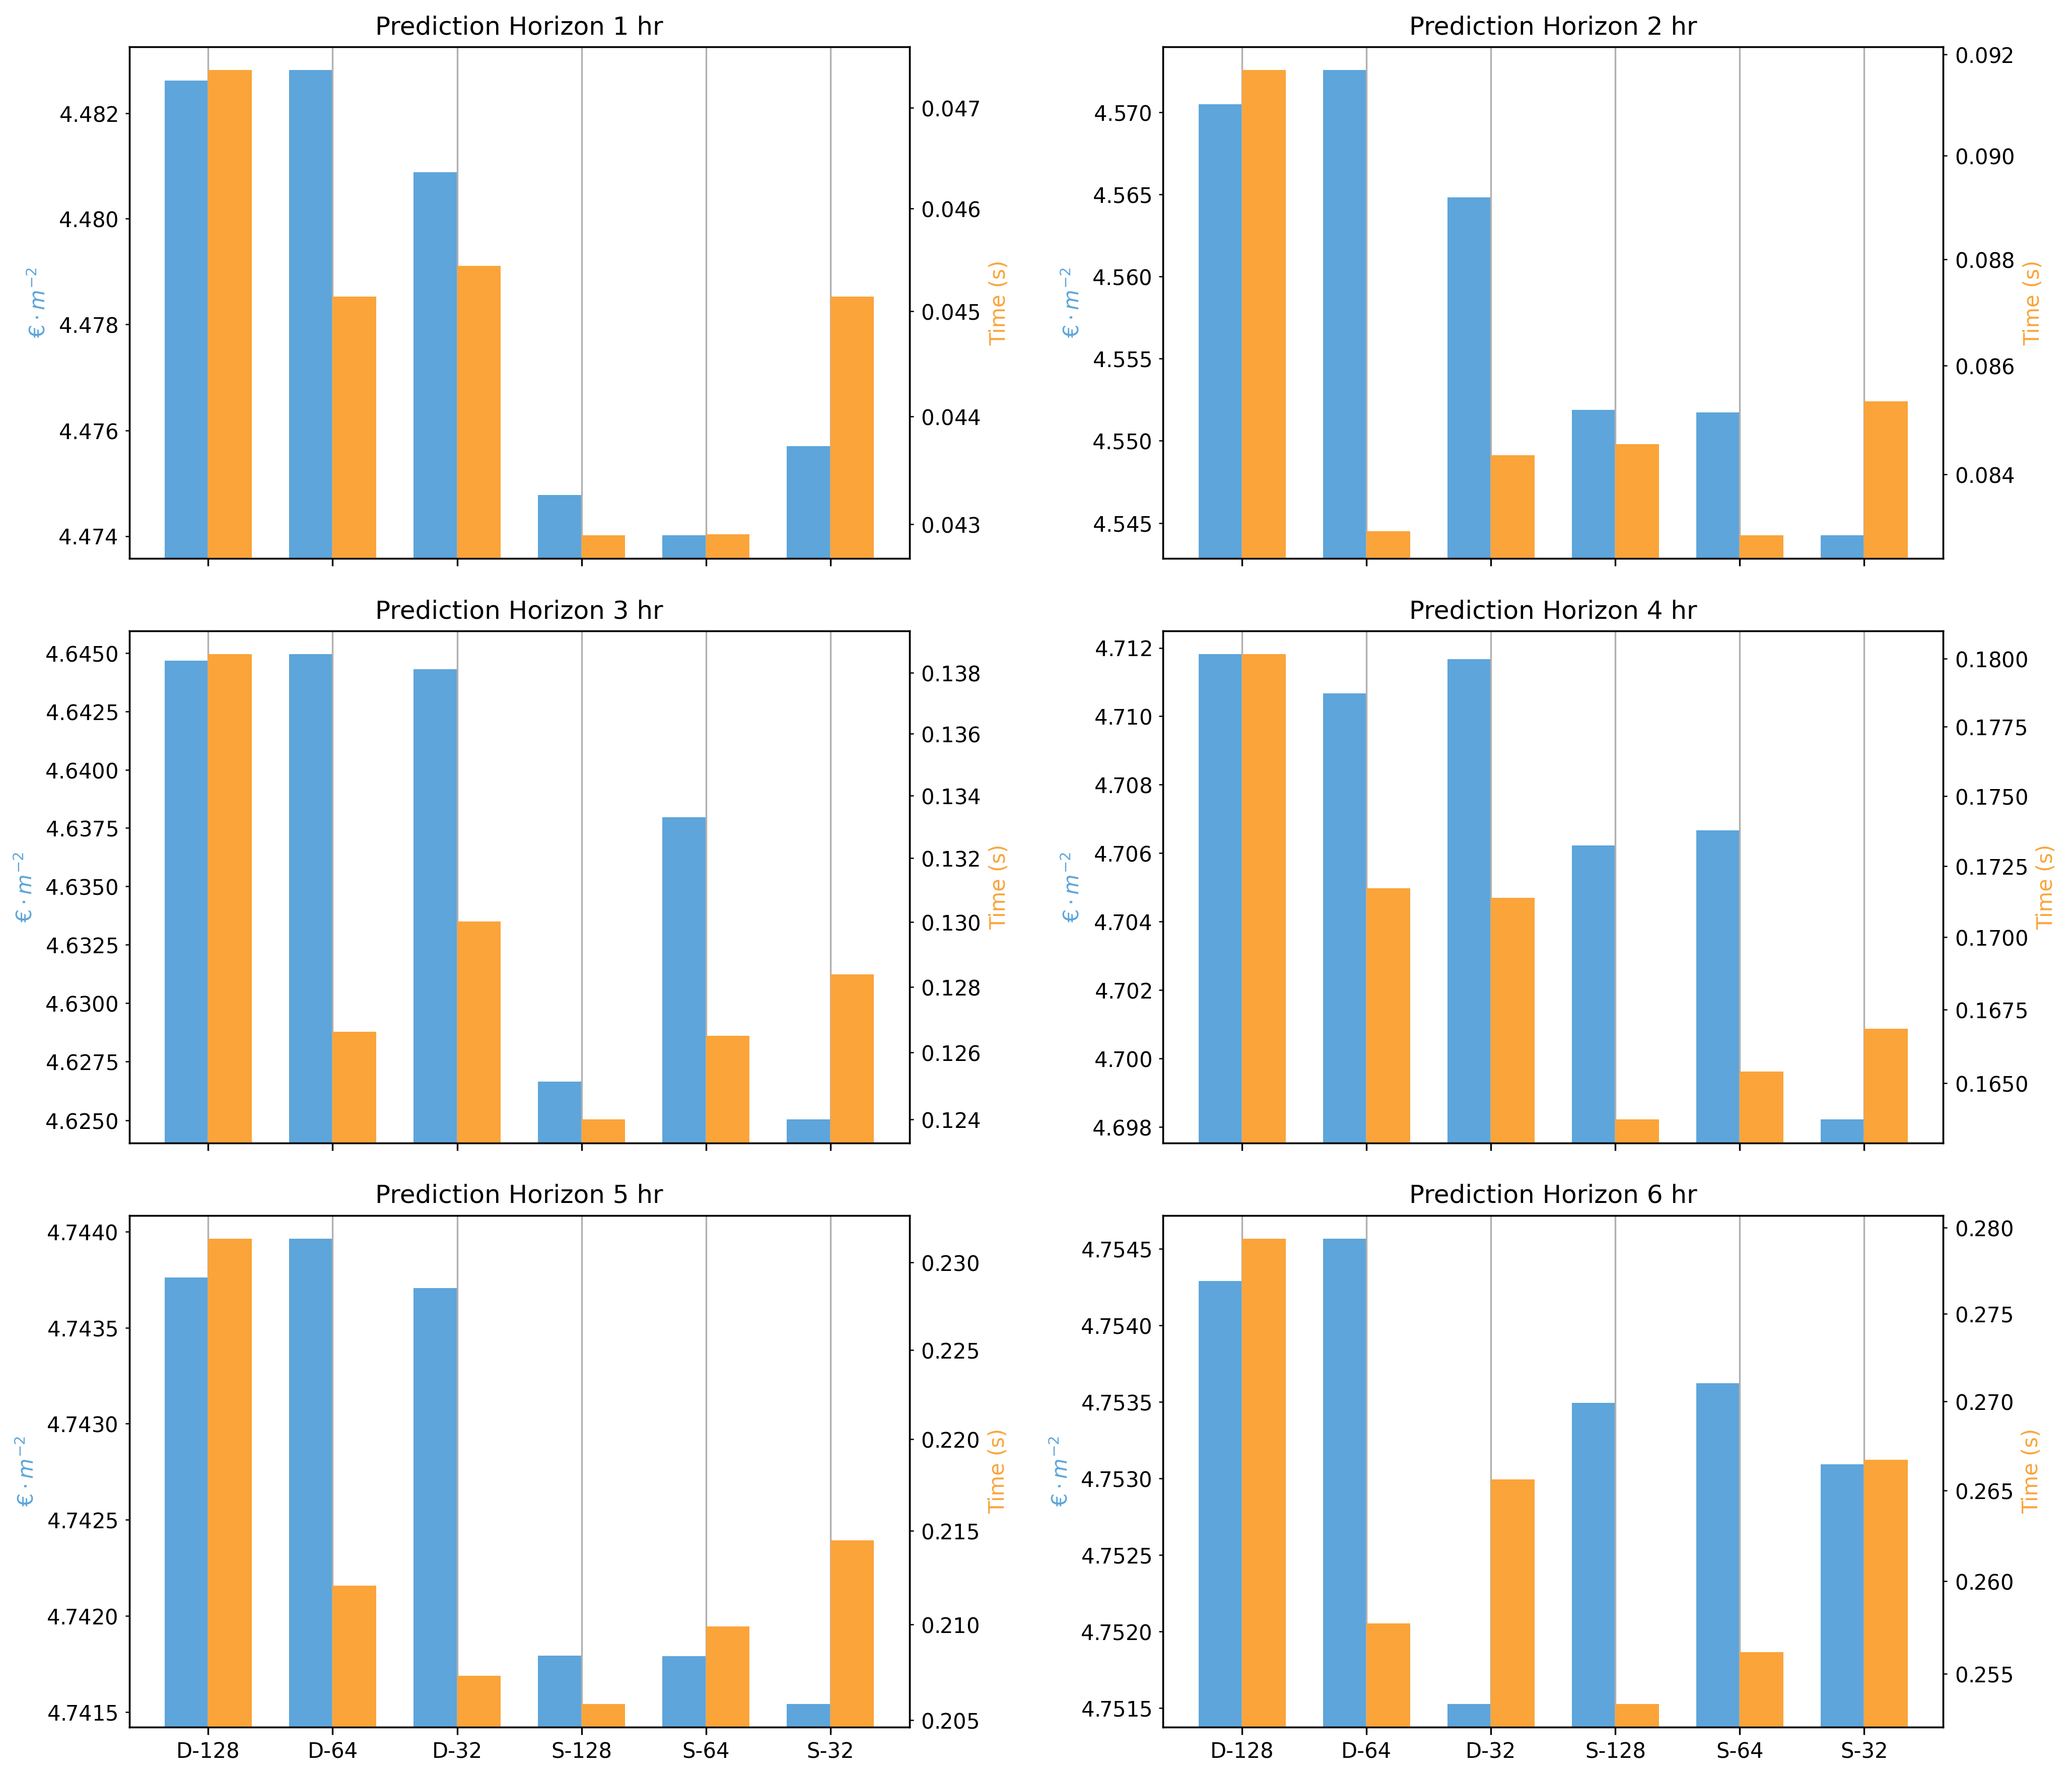
\includegraphics[width=\textwidth]{figures/speed_up_neurons_bar_graph.png}
	\caption{Fast RL-MPC with Reduced Neurons}
	\label{fig:neurons-speedup-bar-graph}
\end{figure}

\section{Case Study 2 - Taylor Approximation}
\emph{results and disucssion of using order 1 and 2 of a taylor approximation of the value function}


\begin{figure}[H]
	\centering
	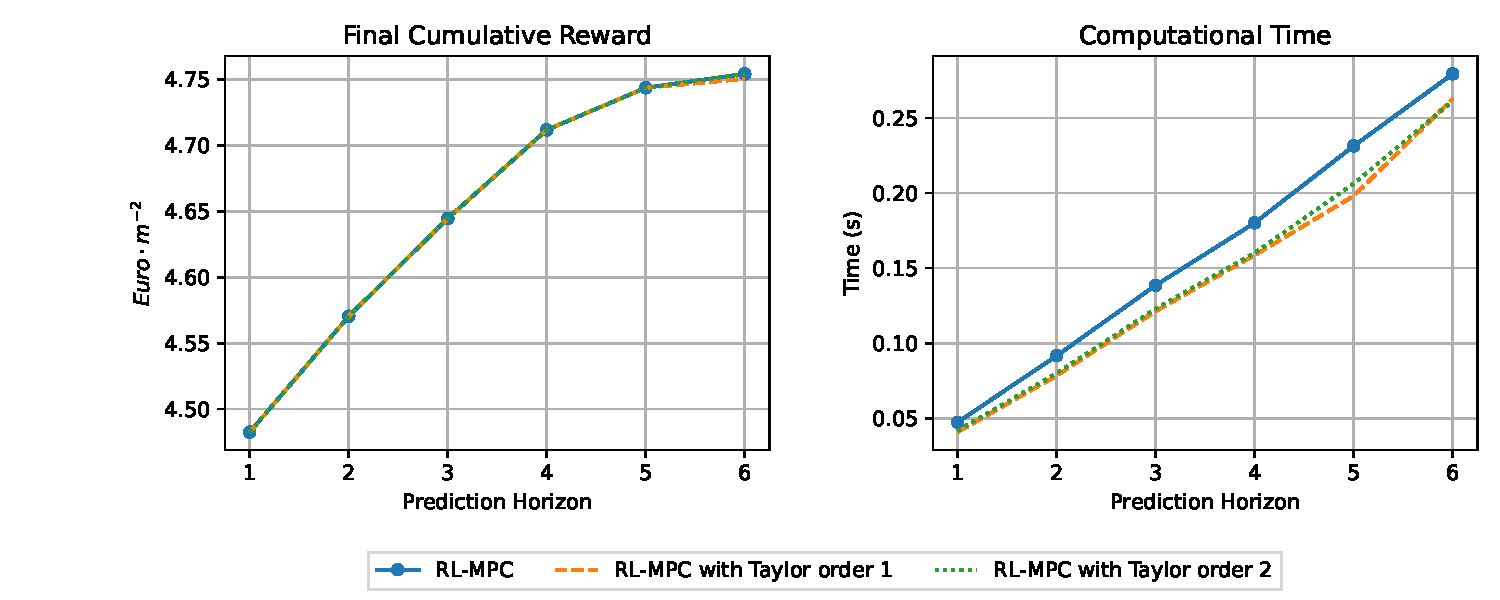
\includegraphics[width=\textwidth]{figures/taylor_speed_up.eps}
	\caption{Fast RL-MPC with Taylor Expansion}
	\label{fig:taylor-speedup}
\end{figure}


\section{Final Result and Conclusion}

\begin{figure}[H]
	\centering
	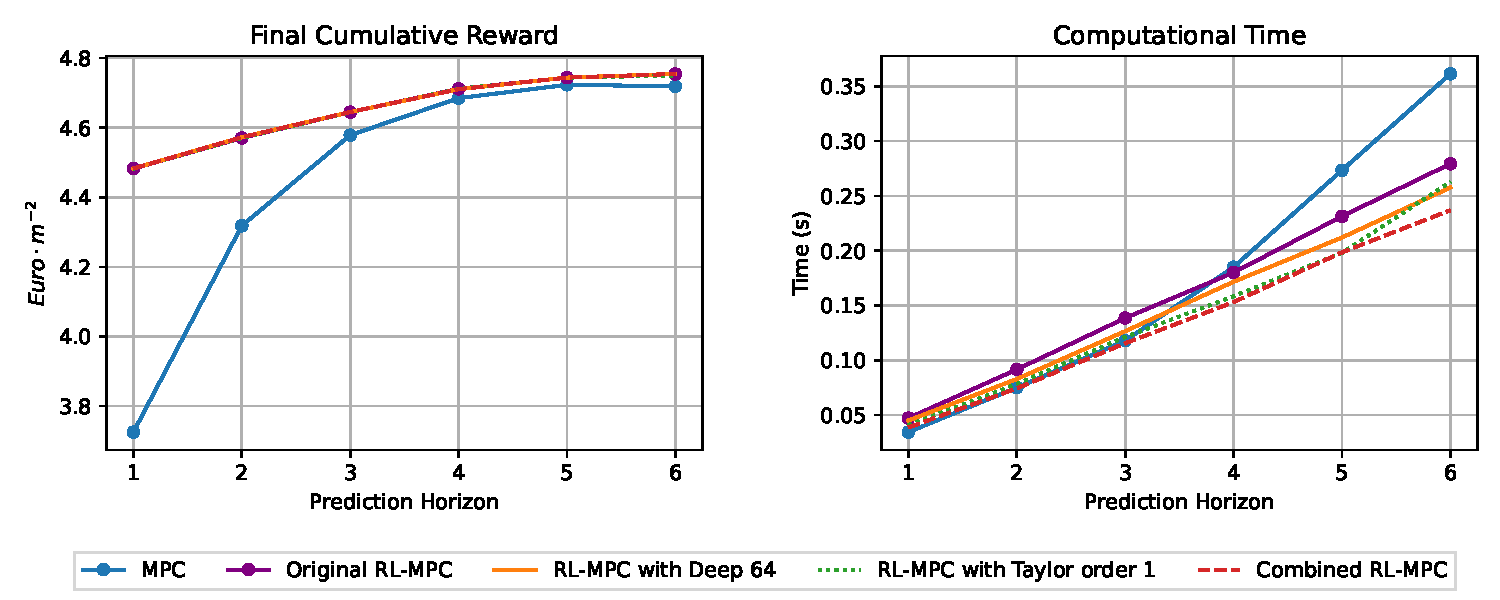
\includegraphics[width=\textwidth]{figures/final_speed_up.eps}
	\caption{Fast RL-MPC}
	\label{fig:final-speedup}
\end{figure}

\emph{A conclusion of the chapter outlining the work done}